\documentclass{article}
\usepackage{enumitem}
\usepackage{amsmath,amssymb,amsthm}
\usepackage{esvect}
\usepackage[letterpaper, margin=1cm]{geometry}
\usepackage{stocktonmacros}
\usepackage{graphicx}
\graphicspath{ {./images/} }

\begin{document}
\begin{enumerate}
  \item Categorize the following equations by:
  \begin{itemize}
    \item Order
    \item Number of independent variables
    \item Linear vs Non-linear. If linear, is it homogeneous or non-homogeneous?
  \end{itemize}
  \begin{enumerate}
    %__________________________________________________________________________%
    \item $u_{xx} + u_{yy} + u_{zz} = f(y, t)$
    \begin{itemize}
      \item Second Order
      \item 4: x, y, z, t
      \item Linear - Non-homogeneous
    \end{itemize}
    %__________________________________________________________________________%
    \item $u_{tt} = u_{tx} + t^2u_x$
    \begin{itemize}
      \item Second Order
      \item 2: x, t
      \item Linear, Homogeneous
    \end{itemize}
    %__________________________________________________________________________%
    \item $(u_y)^4 + (u_x)^5 = 7$
    \begin{itemize}
      \item First Order
      \item 2: x, y
      \item Non-linear
    \end{itemize}
    %__________________________________________________________________________%
    \item $u_t - \sqrt{1 + (u_y)^2} = 0$
    \begin{itemize}
      \item First Order
      \item 2: y, t
      \item Non-linear
    \end{itemize}
    %__________________________________________________________________________%
    \item $u_t + (u^2)_x = 0$
    \begin{itemize}
      \item First order
      \item 2: x, t
      \item Non-linear
    \end{itemize}
    %__________________________________________________________________________%
    \item $u_t + \frac{\p^2}{\p x^2}u^3 - \frac{\p}{\p y}u^{\frac{5}{2}} = 0$
    \begin{itemize}
      \item Second Order
      \item 3: x, y, t
      \item Non-linear
    \end{itemize}
    %__________________________________________________________________________%
    \item $u_t - u u_y + 6 u_{xx} = 4 \cos t$
    \begin{itemize}
      \item Second Order
      \item 3: x, y, t
      \item Non-linear
    \end{itemize}
    %__________________________________________________________________________%
    \item $0 = \grad \cdot \grad u$ (Where $u$ is dependent on $n$ variables $x_1, x_2, \ldots, x_n$).
    \begin{align*}
      0 & = \frac{\p^2 u}{\p x^2_1} + \frac{p^2 u}{\p x^2_2} + \ldots + \frac{p^2 u}{\p x^2_n}
    \end{align*}
    \begin{itemize}
      \item Second Order
      \item $n$ variables.
      \item Linear, homogeneous
    \end{itemize}
    %__________________________________________________________________________%
    \item $\Big( \frac{\p^4 u}{\p t \p x^2 \p y} \Big)^2 = g(x, t)$
    \begin{itemize}
      \item Fourth order
      \item 3: x, y, t
      \item Non-linear
    \end{itemize}
    %__________________________________________________________________________%
    \item $u_t = \frac{u_{xx} (u_y)^2 - 2 u_x u_y u_{xy} + u_{yy} (u_x)^2}{(u_y)^2 + (u_x)^2} $
    \begin{itemize}
      \item Second Order
      \item 2: x, y
      \item Non-linear
    \end{itemize}
    %__________________________________________________________________________%
    \item $\sqrt{u_x + u_y} = e^{xt}$
    \begin{itemize}
      \item First Order
      \item 3: x, y, t
      \item Non-linear
    \end{itemize}
  \end{enumerate}
  \newpage
  \item Derive the heat equation for a 2-D region in the following ways:
  \begin{enumerate}
    \item Do this over a differential square $\Delta x \Delta y$, generalizing the argument from the notes.

    Let us derive the heat equation for a 2-D region. We want to consider the conservation of energy where we can consider heat accumulated with heat in - heat out. Let us consider the transfer of heat about the x axis:
    \begin{align}
      q_{1}(x, y, t) \Delta y \Delta z \Delta t
    \end{align}
    Here, we want to consider finding the heat accumulated through the heat in and heat out, therefore we want to consider $x_0$ and $x_0 + \Delta$
    %
    \begin{align}
      q_1(x_0, y, t) \Delta y \Delta z \Delta t - q_1(x_0 + \Delta x, y, t) \Delta y \Delta z \Delta t
    \end{align}
    Here, we want to consider the deltas in 2). We have our heat function in the $x$ direction, $q_1$. We have a function with variables $y, t$. Instead of keeping them in their form, let us find the integral and integrate in terms of $y$ and $t$:
    %
    \begin{align}
      \Delta z \int \int q_1(x_0, y, t) \text{dy} \text{dt} - \Delta z \int \int q_1(x_0 + \Delta x, y, t) \text{dy} \text{dt}
    \end{align}

    Let us take note of the integral. We are finding the area over the span of $y$ and $t$, these are our intervals. In addition, let us combine the integrals:
    %
    \begin{align}
      \Delta z \int^{t_0 + \Delta t}_{t_0} \int^{y_0 + \Delta y}_{y_0} q_1(x_0, y, t) - q_1(x_0 + \Delta x, y, t) \text{ dy dt}
    \end{align}

    Now for the $y$ direction, we can repeat the previous steps to obtain the following equation:
    %
    \begin{align}
      \Delta z \int^{t_0 + \Delta t}_{t_0} \int^{x_0 + \Delta x}_{x_0} q_2(x, y_0, t) - q_2(x, y_0 + \Delta y, t) \text{ dx dt}
    \end{align}

    Now, let us combine both equations:
    %
    \begin{align}
      \Delta z \int^{t_0 + \Delta t}_{t_0} \int^{y_0 + \Delta y}_{y_0} q_1(x_0, y, t) - q_1(x_0 + \Delta x, y, t) \text{ dy dt} + \Delta z \int^{t_0 + \Delta t}_{t_0} \int^{x_0 + \Delta x}_{x_0} q_2(x, y_0, t) - q_2(x, y_0 + \Delta y, t) \text{ dx dt}
    \end{align}
    Before moving forward, let us break our equation into two parts to keep our equation manipulation on one line. We will break the equation where both terms are added together.
    %
    \begin{enumerate}
      \item Let us consider the first half of our equation:
      \begin{align}
        \Delta z \int^{t_0 + \Delta t}_{t_0} \int^{y_0 + \Delta y}_{y_0} q_1(x_0, y, t) - q_1(x_0 + \Delta x, y, t) \text{ dy dt}\\
      \end{align}
      Now, while keeping in mind the manipulations must be the same as in line (9), let us multiply by\\
      $\displaystyle \lim_{\Delta x, \Delta y, \Delta t \to 0} \frac{1}{\Delta x \Delta y \Delta z \Delta t}$.
      \begin{align}
        \lim_{\Delta x, \Delta y, \Delta t \to 0} \frac{1}{\Delta x \Delta y \Delta z \Delta t} \left(\Delta z \int^{t_0 + \Delta t}_{t_0} \int^{y_0 + \Delta y}_{y_0} q_1(x_0, y, t) - q_1(x_0 + \Delta x, y, t) \text{ dy dt}\right)\\
        \lim_{\Delta x, \Delta y, \Delta t \to 0} \frac{1}{\Delta x \Delta y \Delta t} \left(\int^{t_0 + \Delta t}_{t_0} \int^{y_0 + \Delta y}_{y_0} q_1(x_0, y, t) - q_1(x_0 + \Delta x, y, t) \text{ dy dt}\right)
      \end{align}
      Here, we want to move $\frac{1}{\Delta x}$ into our integral.
      \begin{align}
        \lim_{\Delta x, \Delta y, \Delta t \to 0} \frac{1}{\Delta y \Delta t} \left(\int^{t_0 + \Delta t}_{t_0} \int^{y_0 + \Delta y}_{y_0} \frac{q_1(x_0, y, t) - q_1(x_0 + \Delta x, y, t)}{\Delta x} \text{ dy dt}\right)
      \end{align}
      Here, we want to move one of our limits to the inside of our integral.
      \begin{align}
        \lim_{\Delta y, \Delta t \to 0} \frac{1}{\Delta y \Delta t} \left(\int^{t_0 + \Delta t}_{t_0} \int^{y_0 + \Delta y}_{y_0}
        \lim_{\Delta x \to 0} \frac{q_1(x_0, y, t) - q_1(x_0 + \Delta x, y, t)}{\Delta x} \text{ dy dt}\right)
      \end{align}
      Here, let us note that the inner integral looks familiar. We can see the inner integral is a difference quotient. However, the fraction is almost the same as the difference quotient, the signs in the numerator are flipped. Here, let us rewrite the fraction as $-q_{1x}$.
      \begin{align}
        \lim_{\Delta y, \Delta t \to 0} \frac{1}{\Delta y \Delta t} \left(\int^{t_0 + \Delta t}_{t_0} \int^{y_0 + \Delta y}_{y_0}
        -q_{1x} \text{ dy dt}\right)
      \end{align}
      \item Let us consider the second half of our equation:
      \begin{align}
        \Delta z \int^{t_0 + \Delta t}_{t_0} \int^{x_0 + \Delta x}_{x_0} q_2(x, y_0, t) - q_2(x, y_0 + \Delta y, t) \text{ dx dt}
      \end{align}
      Now, while keeping in mind the manipulations must be the same as in line (9), let us multiply by\\
      $\displaystyle \lim_{\Delta x, \Delta y, \Delta t \to 0} \frac{1}{\Delta x \Delta y \Delta z \Delta t}$.
      \begin{align}
        \lim_{\Delta x, \Delta y, \Delta t \to 0} \frac{1}{\Delta x \Delta y \Delta z \Delta t} \left(\Delta z \int^{t_0 + \Delta t}_{t_0} \int^{x_0 + \Delta x}_{x_0} q_2(x, y_0, t) - q_2(x, y_0 + \Delta y, t) \text{ dx dt}\right)\\
        \lim_{\Delta x, \Delta y, \Delta t \to 0} \frac{1}{\Delta x \Delta y \Delta t} \left(\int^{t_0 + \Delta t}_{t_0} \int^{x_0 + \Delta x}_{x_0} q_2(x, y_0, t) - q_2(x, y_0 + \Delta y, t) \text{ dx dt}\right)
      \end{align}
      Here, we want to move $\frac{1}{\Delta y}$ into our integral.
      \begin{align}
        \lim_{\Delta x, \Delta y, \Delta t \to 0} \frac{1}{\Delta x \Delta t} \left(\int^{t_0 + \Delta t}_{t_0} \int^{x_0 + \Delta x}_{x_0} \frac{q_2(x, y_0, t) - q_2(x, y_0 + \Delta y, t)}{\Delta y} \text{ dx dt}\right)
      \end{align}
      Here, we want to move one of our limits to the inside of our integral.
      \begin{align}
        \lim_{\Delta x, \Delta t \to 0} \frac{1}{\Delta x \Delta t} \left(\int^{t_0 + \Delta t}_{t_0} \int^{x_0 + \Delta x}_{x_0}
        \lim_{\Delta y \to 0} \frac{q_2(x, y_0, t) - q_2(x, y_0 + \Delta y, t)}{\Delta y} \text{ dx dt}\right)
      \end{align}
      Here, let us note that the inner integral looks familiar. We can see the inner integral is a difference quotient. However, the fraction is almost the same as the difference quotient, the signs in the numerator are flipped. Here, let us rewrite the fraction as $-q_{2y}$.
      \begin{align}
        \lim_{\Delta x, \Delta t \to 0} \frac{1}{\Delta x \Delta t} \left(\int^{t_0 + \Delta t}_{t_0} \int^{x_0 + \Delta x}_{x_0}
        -q_{2y} \text{ dx dt}\right)
      \end{align}
    \end{enumerate}
    Here, let us combine lines 13 and 19:
    \begin{align}
      \lim_{\Delta y, \Delta t \to 0} \frac{1}{\Delta y \Delta t} \left(\int^{t_0 + \Delta t}_{t_0} \int^{y_0 + \Delta y}_{y_0}
      -q_{1x} \text{ dy dt}\right) +
      \lim_{\Delta x, \Delta t \to 0} \frac{1}{\Delta x \Delta t} \left(\int^{t_0 + \Delta t}_{t_0} \int^{x_0 + \Delta x}_{x_0}
      -q_{2y} \text{ dx dt}\right)
    \end{align}
    Here, let us assess our limit and integral:
    \begin{align}
      \lim_{\Delta t \to 0} \frac{1}{\Delta t} \left(\int^{t_0 + \Delta t}_{t_0}
      -q_{1x}(x_0, y_0 + \Delta y) \text{ dt}\right) + &
      \lim_{\Delta t \to 0} \frac{1}{\Delta x \Delta t} \left(\int^{t_0 + \Delta t}_{t_0}
      -q_{2y}(x_0 + \Delta x, y_0, t) \text{ dt}\right)\\
      %
      \lim_{\Delta y, \Delta t \to 0}
      -q_{1x}(x_0, y_0 + \Delta y, t_0 + \Delta t) + &
      \lim_{\Delta x, \Delta t \to 0}
      -q_{2y}(x_0 + \Delta x, y_0, t_0 + \Delta t)
    \end{align}

    Here, let us take our limit:
%
    \begin{align}
      -q_{1x}(x_0, y_0, t_0) + &
      -q_{2y}(x_0, y_0, t_0)
    \end{align}

    Now from here, we want to look at the right side of our equation. First, we looked at the heat through the $x$ and $y$ direction, next we want to look at the heat accumulated over time. Here, let us first look at the $x$ direction. Let us consider the following equation:
%
    \begin{align}
      \Delta z
      \int \int Q_1(x_0 + \Delta x, y, t_0 + \Delta t) \text{ dx dt} - \int \int Q_1(x_0 + \Delta x, y, t_0 + \Delta t) \text{ dx dt}
    \end{align}

    Here, we want to find our heat energy density over the span of time and the $x$ space.
%
    \begin{align}
      \Delta z
      \int^{x_0 + \Delta x}_{x_0}
      \int^{t_0 + \Delta t}_{t_0}
      Q_1(x_0 + \Delta x, y, t_0 + \Delta t) \text{ dx dt} - \Delta z \int^{t_0 + \Delta t}_{t_0} \int^{x_0 + \Delta x}_{x_0} Q_1(x_0 + \Delta x, y, t_0 + \Delta t) \text{ dt dx}
    \end{align}

    Here, we can combine both integrals.
%
    \begin{align}
      \Delta z
      % First integral
      \int^{x_0 + \Delta x}_{x_0}
      % Second integral
      \int^{t_0 + \Delta t}_{t_0}
      % First term
      Q_1(x+\Delta x, y, t_0 + \Delta t) -
      % Second term
      Q_1(x+\Delta x, y, t_0 + \Delta t)
      %
      \text{ dt dx}
    \end{align}

    From here, we follow the same manipulation as we did at line 9,
%
    \begin{align}
      \lim_{\Delta x, \Delta y, \Delta t \to 0} \frac{1}{\Delta x \Delta y \Delta z \Delta t}
      \Delta z
      % First integral
      \int^{x_0 + \Delta x}_{x_0}
      % Second integral
      \int^{t_0 + \Delta t}_{t_0}
      % First term
      & Q_1(x_0 + \Delta x, y, t_0 + \Delta t) -
      % Second term
      Q_1(x_0 + \Delta x, y, t_0 + \Delta t)
      %
      \text{ dt dx}\\
      %
      \lim_{\Delta y \to 0} \frac{1}{\Delta y}
      % First integral
      \int^{x_0 + \Delta x}_{x_0}
      % Second integral
      \int^{t_0 + \Delta t}_{t_0}
      % Limit
      \lim_{\Delta x, \Delta t \to 0}
      % First term
      & \frac{
      Q_1(x_0 + \Delta x, y, t_0 + \Delta t) -
      % Second term
      Q_1(x_0 + \Delta x, y, t_0 + \Delta t)
      }
      {\Delta x \Delta t}
      %
      \text{ dt dx}
    \end{align}

    Now, on the right side, we see we have the difference quotient.
    %
    \begin{align}
      \lim_{\Delta y \to 0}
      \frac{1}{\Delta y}
      \int^{y_0 + \Delta y}_{y_0}
      & Q_{xt}(x_0, y, t_0) \text{ dy}\\
      %
      \lim_{\Delta y \to 0}
      & Q_{xt}(x_0, y_0 + \Delta y, t_0)\\
      %
      & Q_{xt}(x_0, y_0, t_0)
    \end{align}

    Following the same steps, we can reach the same term when we start in the $y$ direction.
    %
    \begin{align}
      Q_{yt}(x_0, y_0, t_0)
    \end{align}

    When we combine the terms together, we get:
    %
    \begin{align}
      Q_{xt}(x_0, y_0, t_0) + Q_{yt}(x_0, y_0, t_0)
    \end{align}

    Now, if we combine lines 23 and 33, we get the following:
%
    \begin{align}
      -q_{1x}(x_0, y_0, t_0) +
      -q_{2y}(x_0, y_0, t_0) & =
      Q_{xt}(x_0, y_0, t_0) +
      Q_{yt}(x_0, y_0, t_0)
    \end{align}

    Since the starting points are arbitrary, let us write:
    %
    \begin{align}
      -q_{1x}(x, y, t) +
      -q_{2y}(x, y, t) & =
      Q_{xt}(x, y, t) +
      Q_{yt}(x, y, t)
    \end{align}
    \item Do this over any small area by using the divergence theorem.

    Let us consider the divergence theorem:

    \begin{align}
      \int \int_R \grad \cdot \vv q \text{ da} & = \oint \vv q \cdot \vv n \text{ dA}
    \end{align}

    Now, let us consider the small area the problem is asking for. Let us consider the force the heat exerts from a region:

    \begin{center}
      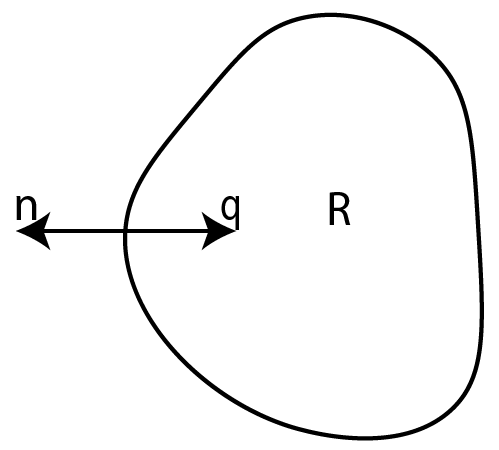
\includegraphics{p2p2}
    \end{center}

    Here, let us find the area of our circle. We can do this by taking the contour integral of the region.

    Let us also consider the direction of the heat flow in vector form. Using what we found at line 35, let us write the following:
%
    \begin{align}
      Q_t(x, y, t) & \Rightarrow \int \int_R Q_t \text{ dA}
    \end{align}

  Now, our goal is to find the heat from the region presented above. We can express our heat from the boundary as the following:
%
  \begin{align}
    \oint_c \vv q \cdot \vv n \text{ ds}
  \end{align}

  Here, using the formula below for a 2-D Divergence Theorem to rewrite our equation:
%
  \begin{align}
    \oint_c \vv q \cdot \vv n \text{ ds} & =
    \int \int_R \grad \cdot \vv F \text{ dA}
  \end{align}

  Do note, however, since our normal force is outwards, we negate the terms:
%
  \begin{align}
      -\oint_c \vv q \cdot \vv n \text{ ds} & = -
      \int \int_R \grad \cdot \vv q \text{ dA}
  \end{align}

  Here, both lines 37 and 40 look to define the heat within the area given. Let us set them equal to each other:
%
  \begin{align}
    \int \int_R Q_t(x, y, t) \text{ dA} & =
    - \int \int_R \grad \cdot \vv q \text{ dA}\\
  \end{align}
%
  Here, let us combine both terms on the same side:
  %
  \begin{align}
    \int \int_R Q_t(x, y, t) + \grad \cdot \vv q \text{ dA} & = 0
  \end{align}
  %
  Here, we have found the conservation of energy.

\end{enumerate}
\end{enumerate}
\bigskip
\textbf{The Divergence Theorem}
\begin{itemize}
  \item In 3-D: Let $\overrightarrow{F} $ be any vector field, then
  \begin{align*}
    \int \int \int_\Omega \grad \cdot \vv F dV & = \int \int_R \vv F \cdot \vv n \text{ dA} \vv{f}
  \end{align*}
  where $\Omega$ is any bounded, simple 3-D region, $R$ is the surface of the 3-D region, and $\vv n$ is the unit outward normal.
  \item In 2-D:
  \begin{align}
    \int \int_R \grad \cdot \vv F \text{ da } & = \into \vv F \cdot \vv n \text{ dS}
  \end{align}
  Where $R$ is a simple 2-D region, $C$ is the boundary of the region, and $\vv n$ is the unit normal.
  \item In 1-D: The Funtamental Theorem of Calculus
  \begin{align}
    \int_L \frac{\p f}{\p x} \text{ dx } & = f(b) - f(a)
  \end{align}
  note that here we are integrating along a line segment $L$ which is $[a, b]$
\end{itemize}
%\newpage
%\begin{enumerate}
%  \item
%  cube: %$|/_$\\
%  $q_1 = \_$
%  \begin{align}
%    q_1(x, y, t) \Delta y \Delta z \Delta t
%  \end{align}
%  Here, we have t and y in our function, we cannot multiply Delta y and Delta t %so we multiply by dy and dz, they become the double integrals
%  \begin{align}
%    \Delta z \int^{t_0 + \Delta t}_{t_0} \int_{y_0}^{y_0 + \Delta y} q_1(x_0, %y, t) dy dt
%  \end{align}
%  This is the heat in on the left side of the cube, and heat out is the right %side. $x_0$ is the heat in and $x_{0} + \Delta x$ is the heat out in this %cube.
%
%  Now, we want to change our $q$ to $q_2$ whih is going upwards.
%  \begin{align}
%    q_2(x, y, t) \Delta x \Delta z \Delta t
%  \end{align}
%  Now, we have $x$ and $t$ in the function, so  we repeat the same process.
%
%  Now, we want to consider the other side as heat accumulated,
%  \begin{align}
%    Q \Delta x \Delta y \Delta z
%  \end{align}
%  $Q$ is a function of $x, y$. Here, we want to change $x$ and $y$. We also %want to compute our ending heat - starting heat ($t_0$).
%  \begin{align}
%    \Delta z \int \int Q(x, y, t_0) dx dy
%  \end{align}
%  Refer to January 24 notes
%  Divide by three variables this time around.
%  Get to $-nabla \cdot q = Q_t$.
%  \begin{align}
%    -< \p / \p x , \p / \p y> \cdot < q_1, q_2 >
%  \end{align}
%  \item
%  \begin{align}
%    \int \int Q_t dx dy - \oint_c \vec q \cdot \vec n ds\\
%    - \nabla \cdot \vec q = Q_t\\
%    - \int_R \int \nabla \cdot \vec q da = \int \int_R Q_t DA\\
%    \int \int_R (Q_t + \nabla \cdot \vec q) dA = 0\\
%    \int^b_a f(x) dx = 0
%  \end{align}
%\end{enumerate}
\end{document}
